% !TeX encoding = UTF-8
% !TeX spellcheck = en_GB

\documentclass[fleqn]{scrartcl}

% Package for typography
\usepackage{microtype}
\usepackage{appendix}

% Packages for graphics and figures
\usepackage{graphicx}
\usepackage{booktabs}
\usepackage{multirow}
\usepackage{bigdelim}
\usepackage{flafter}
%\usepackage{floatrow}
\usepackage{rotating}
% https://tex.stackexchange.com/a/77945
\newsavebox\CaptionBoxA
\newsavebox\CaptionBoxB
\newlength\ImgHeight
\newcommand{\twofigs}[6]{ % 
	\begin{figure}[H]
		\vbox to \textheight{%
			\centering
			\setbox\CaptionBoxA=\vbox{%
				\begingroup % color support
				\centering
				\caption{#2}%
				\label{#3}%
				\endgroup
			}
			\setbox\CaptionBoxB=\vbox{%
				\begingroup % color support
				\centering
				\caption{#5}%
				\label{#6}%
				\endgroup
			}
			\setlength{\ImgHeight}{%
				.5\dimexpr\textheight 
				-\ht\CaptionBoxA-\dp\CaptionBoxA
				-\ht\CaptionBoxB-\dp\CaptionBoxB
				-\floatsep
				\relax
			}
			
			
			\includegraphics[height=\ImgHeight,width=\linewidth,keepaspectratio]{#1}
			
			\unvbox\CaptionBoxA
			
			\vspace{\floatsep}
			\vspace{0pt minus .25\floatsep}% glue for safety
			\vspace{0pt plus 1fil}% glue for smaller images 
			\nointerlineskip % interline skip affects the calculation of \ImgHeight
			
			
			\includegraphics[height=\ImgHeight,width=\linewidth,keepaspectratio]{#4}
			
			\unvbox\CaptionBoxB
		}
	\end{figure}
}
\usepackage{tikz}
\usetikzlibrary{shapes,arrows,positioning,shapes.multipart}

% Typeset code
\usepackage{minted}

% Packages for typesetting math
\usepackage{physics}
\usepackage{mathtools}
\usepackage{bm}
\usepackage{siunitx}
\newcommand{\earth}{\oplus}
\newcommand{\sun}{\odot}
\usepackage{chemmacros}
\chemsetup{modules=all}

% Packages for referencing
\usepackage{varioref}
\usepackage[hidelinks]{hyperref}
\usepackage{cleveref}
\usepackage[backend=biber]{biblatex}
\addbibresource{report4.bib}

% Macro for typesetting "C++"
\usepackage{relsize}
\newcommand\cpp{C\nolinebreak[4]\hspace{-.05em}\raisebox{.4ex}{\relsize{-3}{\textbf{++}}}}
% Macro for typesetting big O-notation
\newcommand{\bigO}[1]{\mathcal{O}(#1)}

\renewcommand{\epsilon}{\varepsilon}

\begin{document}
	\title{The basics of molecular dynamics in the microcanonical ensemble}
	\subtitle{\url{https://github.com/sverl/FYS3150-FYS4150}}
	\author{Sverre Løyland}
	\maketitle
	
	\begin{abstract}
		Code to perform molecular dynamics in the microcanonical ensemble has been implemented successfully and used to find the melting point of argon by calculating diffusion constants at different temperatures. The melting point was found to be a bit lower than \SI{320}{K}. 
	\end{abstract}

	\section{Introduction}
	Molecular dynamics is computational method to derive thermodynamic properties of a system. By simulating a system over longer periods (on thermodynamic scale) and sampling quantities, certain properties can be calculated.
	
	This project explores the basics of molecular dynamics, in particular the melting of solid argon. Here, 500 \isotope*{40,Ar} atoms interacting in Lennard-Jones potentials initially in a face-centred cubic lattice are simulated, and the simulation is repeated at different temperatures to derive a melting point.
	
	\section{Theory}
	\subsection{Maxwell-Boltzmann distribution}
	The Maxwell-Boltzmann distributions are the probability distribution of the velocities, speeds and momenta of particles at equilibrium. The distribution assumes uncorrelated velocities and spherical symmetry of the distribution\footnote{Many sources says the particles need to non-interacting except in brief collisions, however this assumption is not necessary.}.
	
	The form of the distribution used in the simulations is the distribution for the velocity given by
	\begin{equation}
		f_v(v_i) = \sqrt{\frac{m}{2\pi k_bT}}e^{-mv_i^2/2k_bT}.
	\end{equation}
	
%	Let $F_v(v_x, v_y, v_z)$ be the probability distribution of the velocity. Because of the spherical symmetry, the distribution can be split into
%	\begin{equation}
%		F_v(v_x, v_y, v_z) = f_v(v_x)f_v(v_y)f_v(v_z)
%	\end{equation}
%	where $f_v(v)$ is the speed distribution. The derivative of $F_v$ can thus be expressed as
%	\begin{align}
%		\pdv{F_v}{v_x} &= \pdv{f_v}{v_x}f_v(v_y)f_v(v_z) \\
%		\pdv{F_v}{v}\pdv{v}{v_x}&= \pdv{f_v}{v_x}f_v(v_y)f_v(v_z) 
%	\shortintertext{Division by $F_v$ gives}
%		\frac{1}{F_v}\pdv{F_v}{v}\pdv{v}{v_x}&= \frac{1}{f_v(v_x)}\pdv{f_v}{v_x} \\
%		\pdv{F_v}{F_v}
%	\end{align}
	
	\subsection{The equipartition theorem}
	The equipartition theorem relates temperature to energy averages. For gas, the theorem says the energy $E$ is related to the temperature $T$ by
	\begin{equation}
		E = T + V = \frac32 Nk_bT+2\pi N\rho\int_0^\infty r^2U(r)g(r)\dd{r}
	\end{equation}
	where $T$ and $V$ are the kinetic and potential energy, $U$ is the (spherical symmetric) interaction potential and $g$ is the radial pair distribution function. 
	
	For an ideal gas where there are no interactions ($U=0,V=0$), this simplifies to	
	\begin{equation}
		E = T = \frac32Nk_b T.
	\end{equation}
	In the simulations, the kinetic energy is assumed to be much bigger than the potential energy so an ideal gas is a good approximation.
	
%	\subsection{Microcanonical ensemble}
	
	\subsection{Lennard-Jones potential}
	The Lennard-Jones potential is a spherically symmetric potential describing the Pauli exchange interaction and London dispersion force. The Pauli exchange interaction is a quantum mechanical effect related to the Pauli exclusion principle and the London dispersion is related to polarisability. The potential is on the form
	\begin{equation}
		U(r) = 4\epsilon\left[\left(\frac{\sigma}{r}\right)^{12}-\left(\frac{\sigma}{r}\right)^6\right]
	\end{equation}
	where $\sigma$ is the zero-point of the potential, i.e approximately how close atoms get) and $\epsilon$ is the depth of the potential at the minimum at $\sqrt[6]{2}\sigma$.

	The parameters can be fitted with experimental values to give a fairly accurate potential which is mathematically and computationally very simple.
	
	The corresponding force is given by
	\begin{align}
		\vb{F} &= -\grad{U(r)} \\
		&= -\dv{U(r)}{r}\frac{\vb{r}}{r} \\
		&= -4\epsilon\left[12\left(\frac{\sigma}{r}\right)^{11}\left(-\frac{\sigma}{r^2}\right)-6\left(\frac{\sigma}{r}\right)^5\left(-\frac{\sigma}{r^2}\right)\right]\frac{\vb{r}}{r} \\
		&= 24\epsilon\left[\left(\frac{\sigma}{r}\right)^{12}-2\left(\frac{\sigma}{r}\right)^6\right]\frac{\vb{r}}{r^2} 
	\end{align}

	\subsection{Einstein diffusion relation}
	The Einstein diffusion relation relates mean square deviation of particle positions to the time by
	\begin{equation}
		\expval{r^2(t)}=6Dt
	\end{equation}
	where $D$ is a diffusion constant varying with temperature. Intuitively, we know the diffusion is a lot lower in solids than in liquids and the diffusion constant is used as an indicator of a phase transition.

	\section{Computational methods}
	\subsection{Scaling}
	By convention, the mass and length units of molecular dynamics are chosen to \SI{1}{amu} and \SI{1}{\angstrom}. The unit of energy is chosen to $\epsilon=\SI{1.65e-21}{J}$ and by using the scale factor $E=k_bT$, the temperature unit becomes \SI{119.8}{K}.
	
	\subsection{Velocity-Verlet integration}
	A mathematically equivalent method to the Verlet method is the velocity-Verlet method. It incorporates the velocities making it self-starting and easily able to output the velocities for other calculations, e.g. kinetic energy.
	
	The velocity-Verlet method is given by
	\begin{align}
		x_{n+1} &= x_n + v_n\Delta t + \frac12 a_n\Delta t^2, \\
		v_{n+1} &= v_n + \frac12\left( a_{n+1} + a_n\right)\Delta t.
	\end{align}
	
	\subsection{Periodic boundary conditions}
	To avoid having to deal with special boundary conditions, periodic boundary conditions are chosen where the potentials are calculated using the minimum image convention, i.e interactions with the closest image of the particle. This also allows in some sense for an simulation box of infinite size. When particle distances become greater than than half the box size in either dimension, the particle image is shifted back into the cell.
	
	However, care has to be taken when calculating properties based on distance such as diffusion. If only the images are saved, the particles can not diffuse more than a cell width in each direction so actual positions have to be calculated as well.
	
	\section{Implementation}
	The molecular dynamics were implemented in \cpp\ based on a partially completed (almost spaghetti-like) code from \href{https://github.com/andeplane/molecular-dynamics-fys3150/tree/b0afed6bd84ecf0230146cc0a808ae6dd0c273e8}{andeplane on Github.com} with some erroneous code. \Cref{fig:flowchart} shows the code flow in the final implementation. The code does not output every integration step as writing to hard disk is slow. This also prevents some correlation in thermodynamic properties. When many simulations were done, the code to write the trajectory file was removed so save even more computation time.
	
	In addition, a script for running the simulations and analysing the results were written in Python 3 to extract the melting point. By linear regression of the mean square deviation over time, a diffusion constant is extracted together with the mean temperature. The diffusion constants are then plotted against the mean temperatures.
	
	\begin{figure}[p]
		\centering
		\tikzstyle{decision} = [diamond, draw, fill=yellow!20, text width=4.5em, text badly centered, inner sep=0pt]
\tikzstyle{block} = [rectangle, draw, fill=blue!20, rounded corners, every text node part/.style={align=left}]
\tikzstyle{end} = [circle, draw, fill=red!20, rounded corners, every text node part/.style={align=left}]
\tikzstyle{line} = [draw, very thick, color=black!50, -latex']
\tikzstyle{cloud} = [draw, ellipse,fill=red!20, node distance=2.5cm, minimum height=2em]

\begin{tikzpicture}[node distance=3.5cm]
	\node [end] (start) {start};
	\node [block, below of=start] (init) {read command line arguments\\
									  	  create face-centered cubic lattice\\
								  	  	  \quad set Maxwell-Boltzmann distribution\\
							  	  	  	  set Lennard-Jones potential\\
						 	  	  	      correct frame of reference\\
							  	  	      first integration step};
	\node [block, below of=init] (verlet) {velocity Verlet integration\\
							   			   update with periodic boundary conditions};
	\node [decision, below of=verlet] (output) {output?};
	\node [decision, below of=output] (last) {last step?};
	\node [end, below of=last] (done) {stop};
	\node [block, left of=output] (print) {sample system\\
										   print stats\\
									  	   print movie frame};

	\path [line] (start) -- (init);
	\path [line] (init) -- (verlet);
	\path [line] (verlet) -- (output);
	\path [line] (output) -- node [near start, above, color=black] {yes} (print);
	\path [line] (last) -- node [near start, left, color=black] {yes} (done);
	\path [line] (output) -- node [near start, left, color=black] {no} (last);
	\path [line] (print) |- (last);
	\path [line] (last) -| node [near start, above, color=black] {no} ++(45mm,0mm) |- (verlet);
\end{tikzpicture}
		\caption{Flowchart for the final implementation of the molecular dynamics simulation.}
		\label{fig:flowchart}	
	\end{figure}
	
	\section{Analysis}
	In each simulation 500 \isotope*{40,Ar} atoms in a face-centred cubic lattice with lattice constance \SI{5.26}{\angstrom} ($\rho=500\cdot\SI{18}{amu}/(5\cdot\SI{5.26}{\angstrom}^3)=\SI{822}{kg/m^3}$) were simulated for \num{5001} integration steps with a time-step of \SI{1}{fs} at a range of different temperatures. First a wide range of temperatures were simulated to find the approximate melting point and then narrower ranges of temperatures were simulated until a satisfactory value could be read off. \Cref{fig:melt} shows the diffusion constants over temperatures. There is a very apparent kink at about \SI{320+-10}{K}. 
	
	\begin{figure}[H]
		\centering
		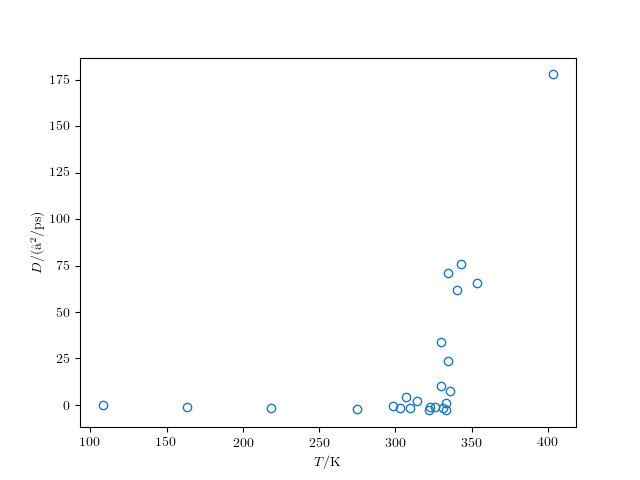
\includegraphics[width=\textwidth]{melt.png}
		\caption{Plot of diffusion constants over temperatures.}
		\label{fig:melt}	
	\end{figure}
	
	The diffusion constants are calculated from linear regression of the whole simulation, not just at equilibrium so if the solid melts at the end of the simulation, only a small diffusion constant is observed or not observed at all if the simulation never reaches equilibrium in the simulation time. This mean the melting point is lower then the kink.
	
	To induce melting and reach equilibrium faster, a set of random atoms can be removed. This is called the voids method. When more and more the atoms are removed, the observed melting points converges to a better estimate.
	
	To get a more accurate melting point range, a simulation in the canonical ensemble where the temperature is varied throughout the simulation can be used, but this requires implementation of a thermo-``stat'' that can adjust the temperature. The melting point can then be estimated from e.g. the density. However, since the temperature is changing, the system never reaches equilibrium and there will be hysteresis. By annealing, a corresponding result can be extracted for the freezing process, but this simulation ``lags'' in the opposite direction so the melting point have to be in-between the observed melting points.
	
	The melting point is difficult to compare to values in the literature as these are usually in the isothermal–isobaric ensemble. To do calculations in the ensemble, both a thermostat and a barostat would need to be implemented.
	
	The relation between the initial temperature and the final temperature is shown in \cref{fig:temps}. As can be seen, the temperature falls to about half of the initial temperature with slight variations depending on the whether the solid melts or not.
	
	\begin{figure}[H]
		\centering
		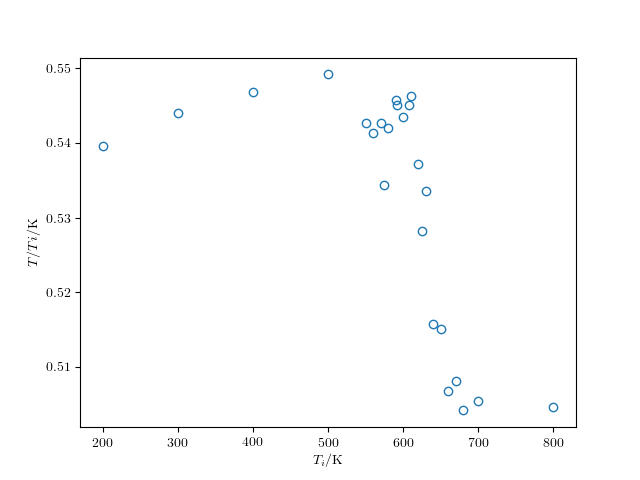
\includegraphics[width=\textwidth]{temp_init.png}
		\caption{Plot of ratio of temperatures and initial temperature over initial temperatures.}
		\label{fig:temps}	
	\end{figure}
	
	\section{Conclusion}
	The desired algorithms were successfully implemented and a melting point extracted. The melting point is probably a bit below \SI{320}{K} for the conditions describes earlier. However, this value does not really represent a usefully quantity as it is in the microcanonical ensemble, but the code serves as a base to build better simulations.
	
	\printbibliography
	
	
\end{document}